\documentclass[12pt]{unlsilabsop}
\title{Module assembly: Gluing of HDI to BBM}
\date{September 24, 2015}
\author{Frank Meier Aeschbacher and José Monroy}
\approved{Frank Meier Aeschbacher}
\sopid{103}
\sopversion{v1}
\sopabstract{Describes the procedures to glue HDI on bare modules using the robotic gantry. The procedure takes place in the clean room.}


\begin{document}

\maketitle

%------------------------------------------------------------------
\section{Scope}
This is a regular part in the manufacturing process of pixel modules at UNL.

%------------------------------------------------------------------
\section{Purpose}
Modules (Sensor + ROCs = BBM) require an additional part to manage the data coming from the sensor; this part, called HDI (High Density Interconect), contains the Token Bit Manager (TBM) and is wired to the ROCs in order to gather and address the data.xs.   

%------------------------------------------------------------------
\section{Definitions}

\begin{itemize}
\item Configuration: The glueing program can be used in 4 configurations
  \begin{enumerate}
  \item glass + polyimide: used for testing purpose; instead of module and HDI, glass and polyimide slides are used.
  \item mocks: used for testing purpose. Module and HDI mocks are used.
  \item HDIV2 + module: for manufacturing modules using HDI V2 (rev B). May be adapted to a new HDI version.
  \item HDIV3 + module: for manufacturing modules using HDI V3 (rev C). May be adapted to a new HDI version.
  \end{enumerate}
\item Fiducials: Reference marks used to define the orientation of the HDIs, modules and tools. Each element has 4 fiducials. 
\item Front panel: It is the window through which the user interact with the software. It show statistical information, status of the vacuum system, tools and elements in use and other information. Some features are:
  \begin{enumerate}
    \item In the main front panel only two step buttons are enabled at a time: the ``step'' button and the finish button. 
    \item Each step has its own front panel. Once the step button is pressed the corresponding front panel appears as a pop-up window and the main front panel becomes locked.
    \item Several pop-up windows appears along the glueing process asking for user inputs, follow the instructions given and/or provide the information needed.
    \item We use 4 elements in the gluing process: Modules (BBM), HDI (HDI), stamp tools (ST) and weight tools (WT). We use the labels in parenthesis to name these elements. We have 4 slots for BBM, 4 slots for HDI, 4 ST (ST1,ST2,...ST4) and 16 WT (WT1, WT2,......WT16). Eventually there will be a pop up window asking for the elements to be used and the mentioned convention is used to identify them.    
  \end{enumerate}
\end{itemize}



%------------------------------------------------------------------
%\section{Responsibilities}

%------------------------------------------------------------------
\section{Equipment}
\begin{center}
\begin{figure}[h]
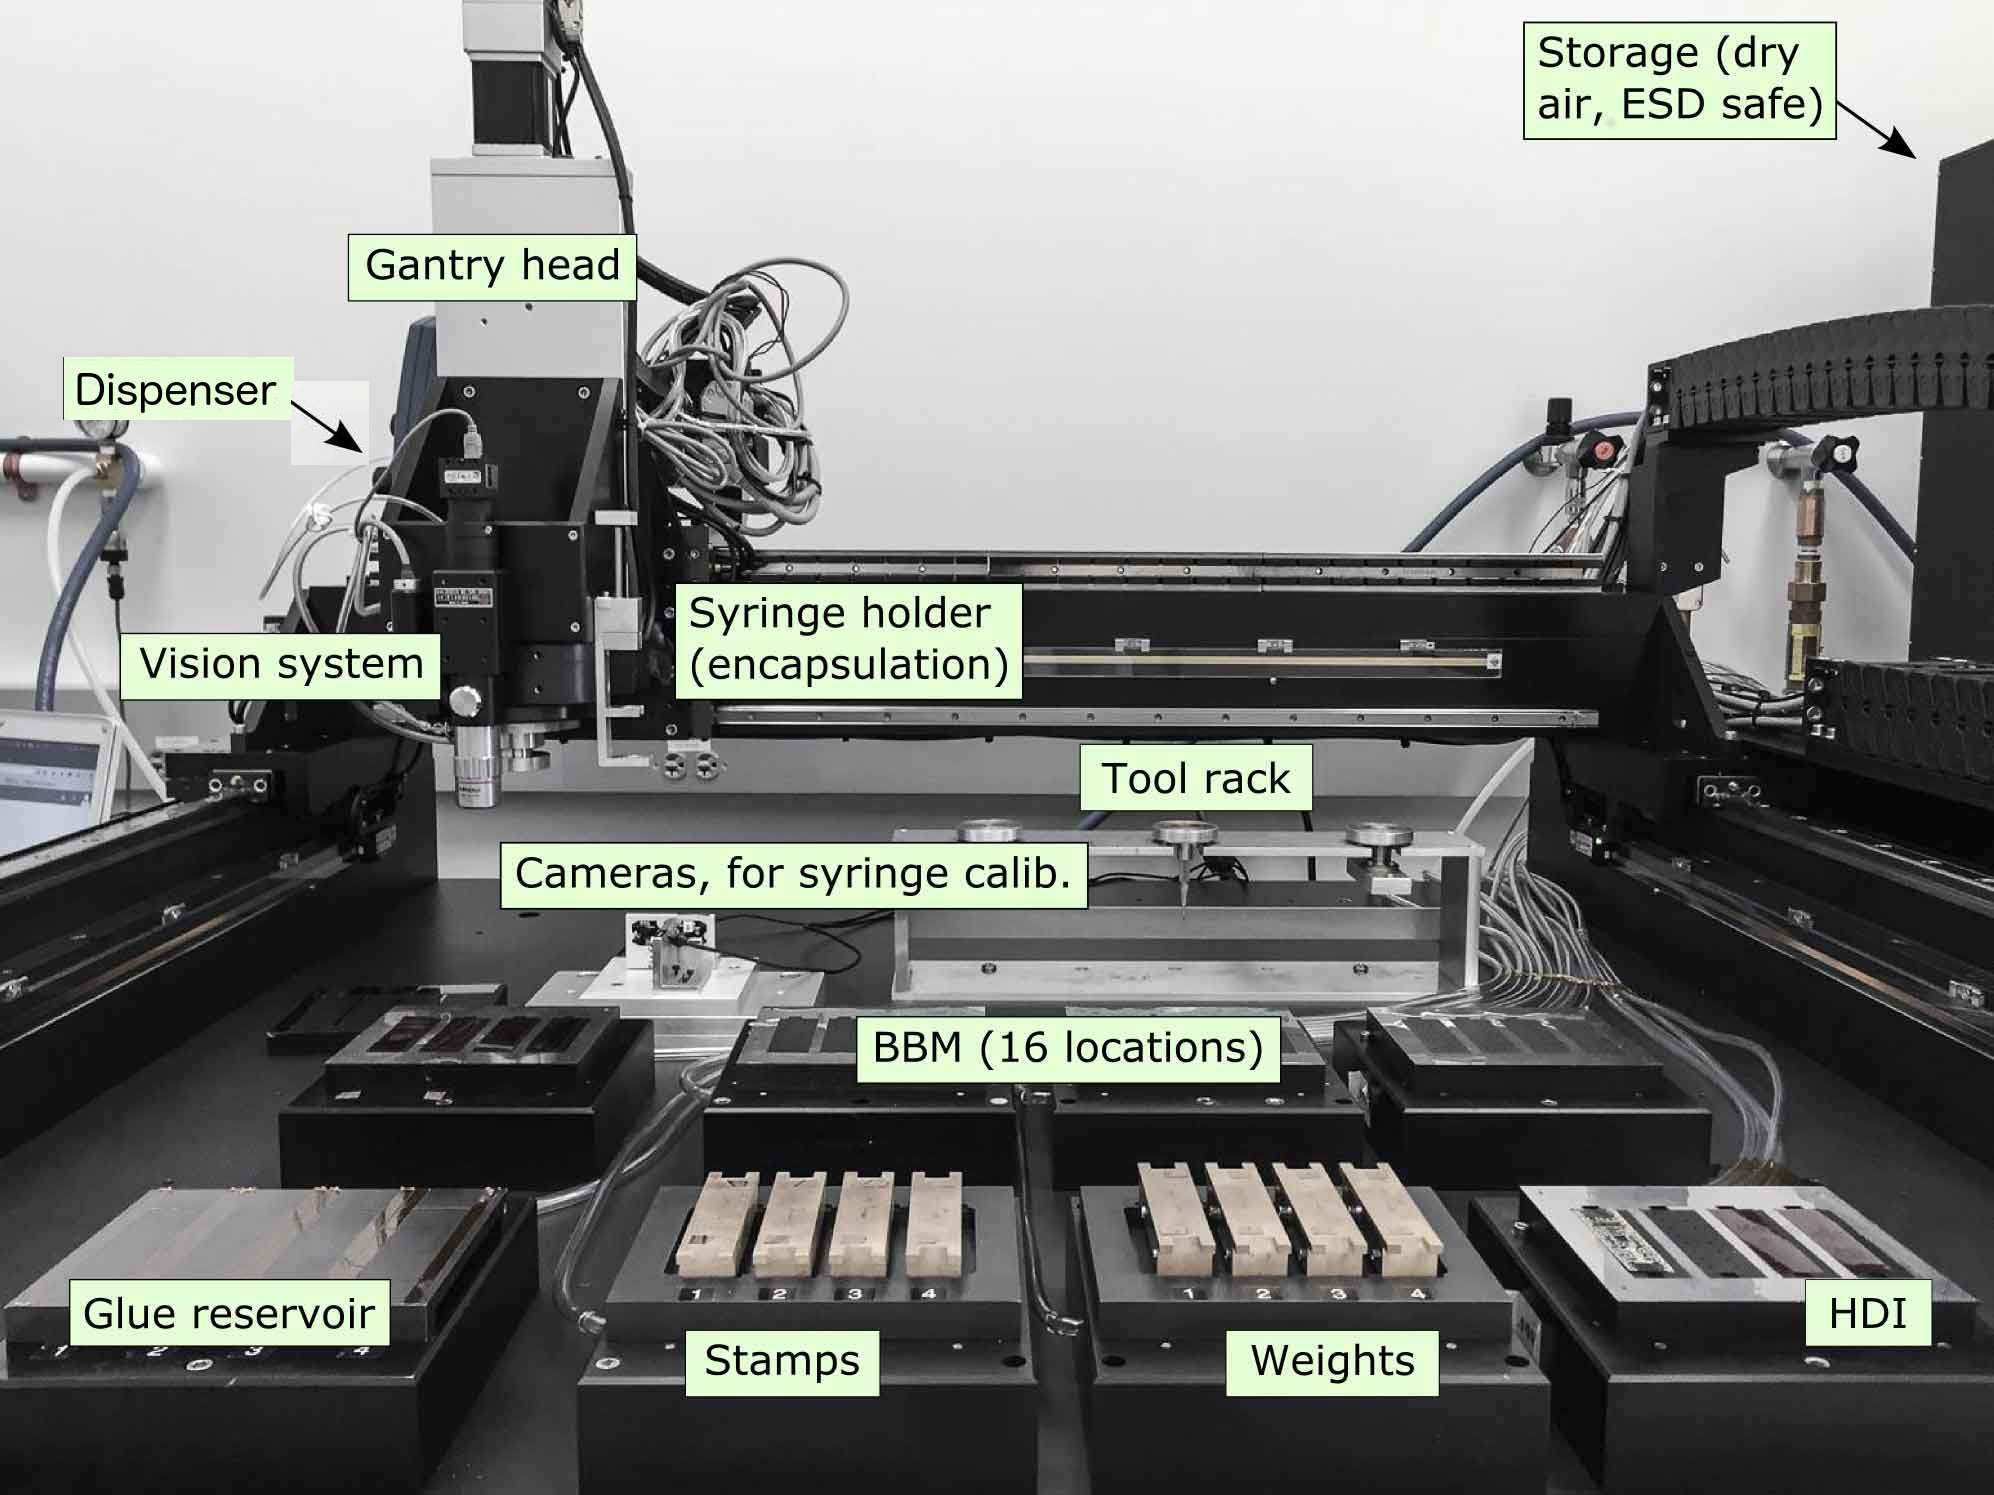
\includegraphics[width=0.9\textwidth]{img/gantryFull16labeled.jpg}
\caption{Gantry setup. Labels indicate the main parts of the setup.}
\label{gantry_setup}
\end{figure}
\end{center}

\begin{itemize}
    \item Gantry
    \item Tools placed on rack: grabber and picker tool (not labeled in the figure  \ref{gantry_setup})
    \item Chucks equipped carrier chucks for BBM, HDI, glue reservoir, stamp tools (ST), and weight tools (WT)
    \item Araldite
    \item Post-It notes, used as surface to mix Araldite
    \item Metallic spatula
    \item PVC squeegee, disposable
    \item Cleaning tools, consisting of brush and 2-Propanole; to clean glue from stamps and reservoir
    \item Felt tip marker, to write batch number on chuck
    \item Vacuum tool to release BBM from GelPak
\end{itemize}

\begin{center}
\begin{figure}[h]
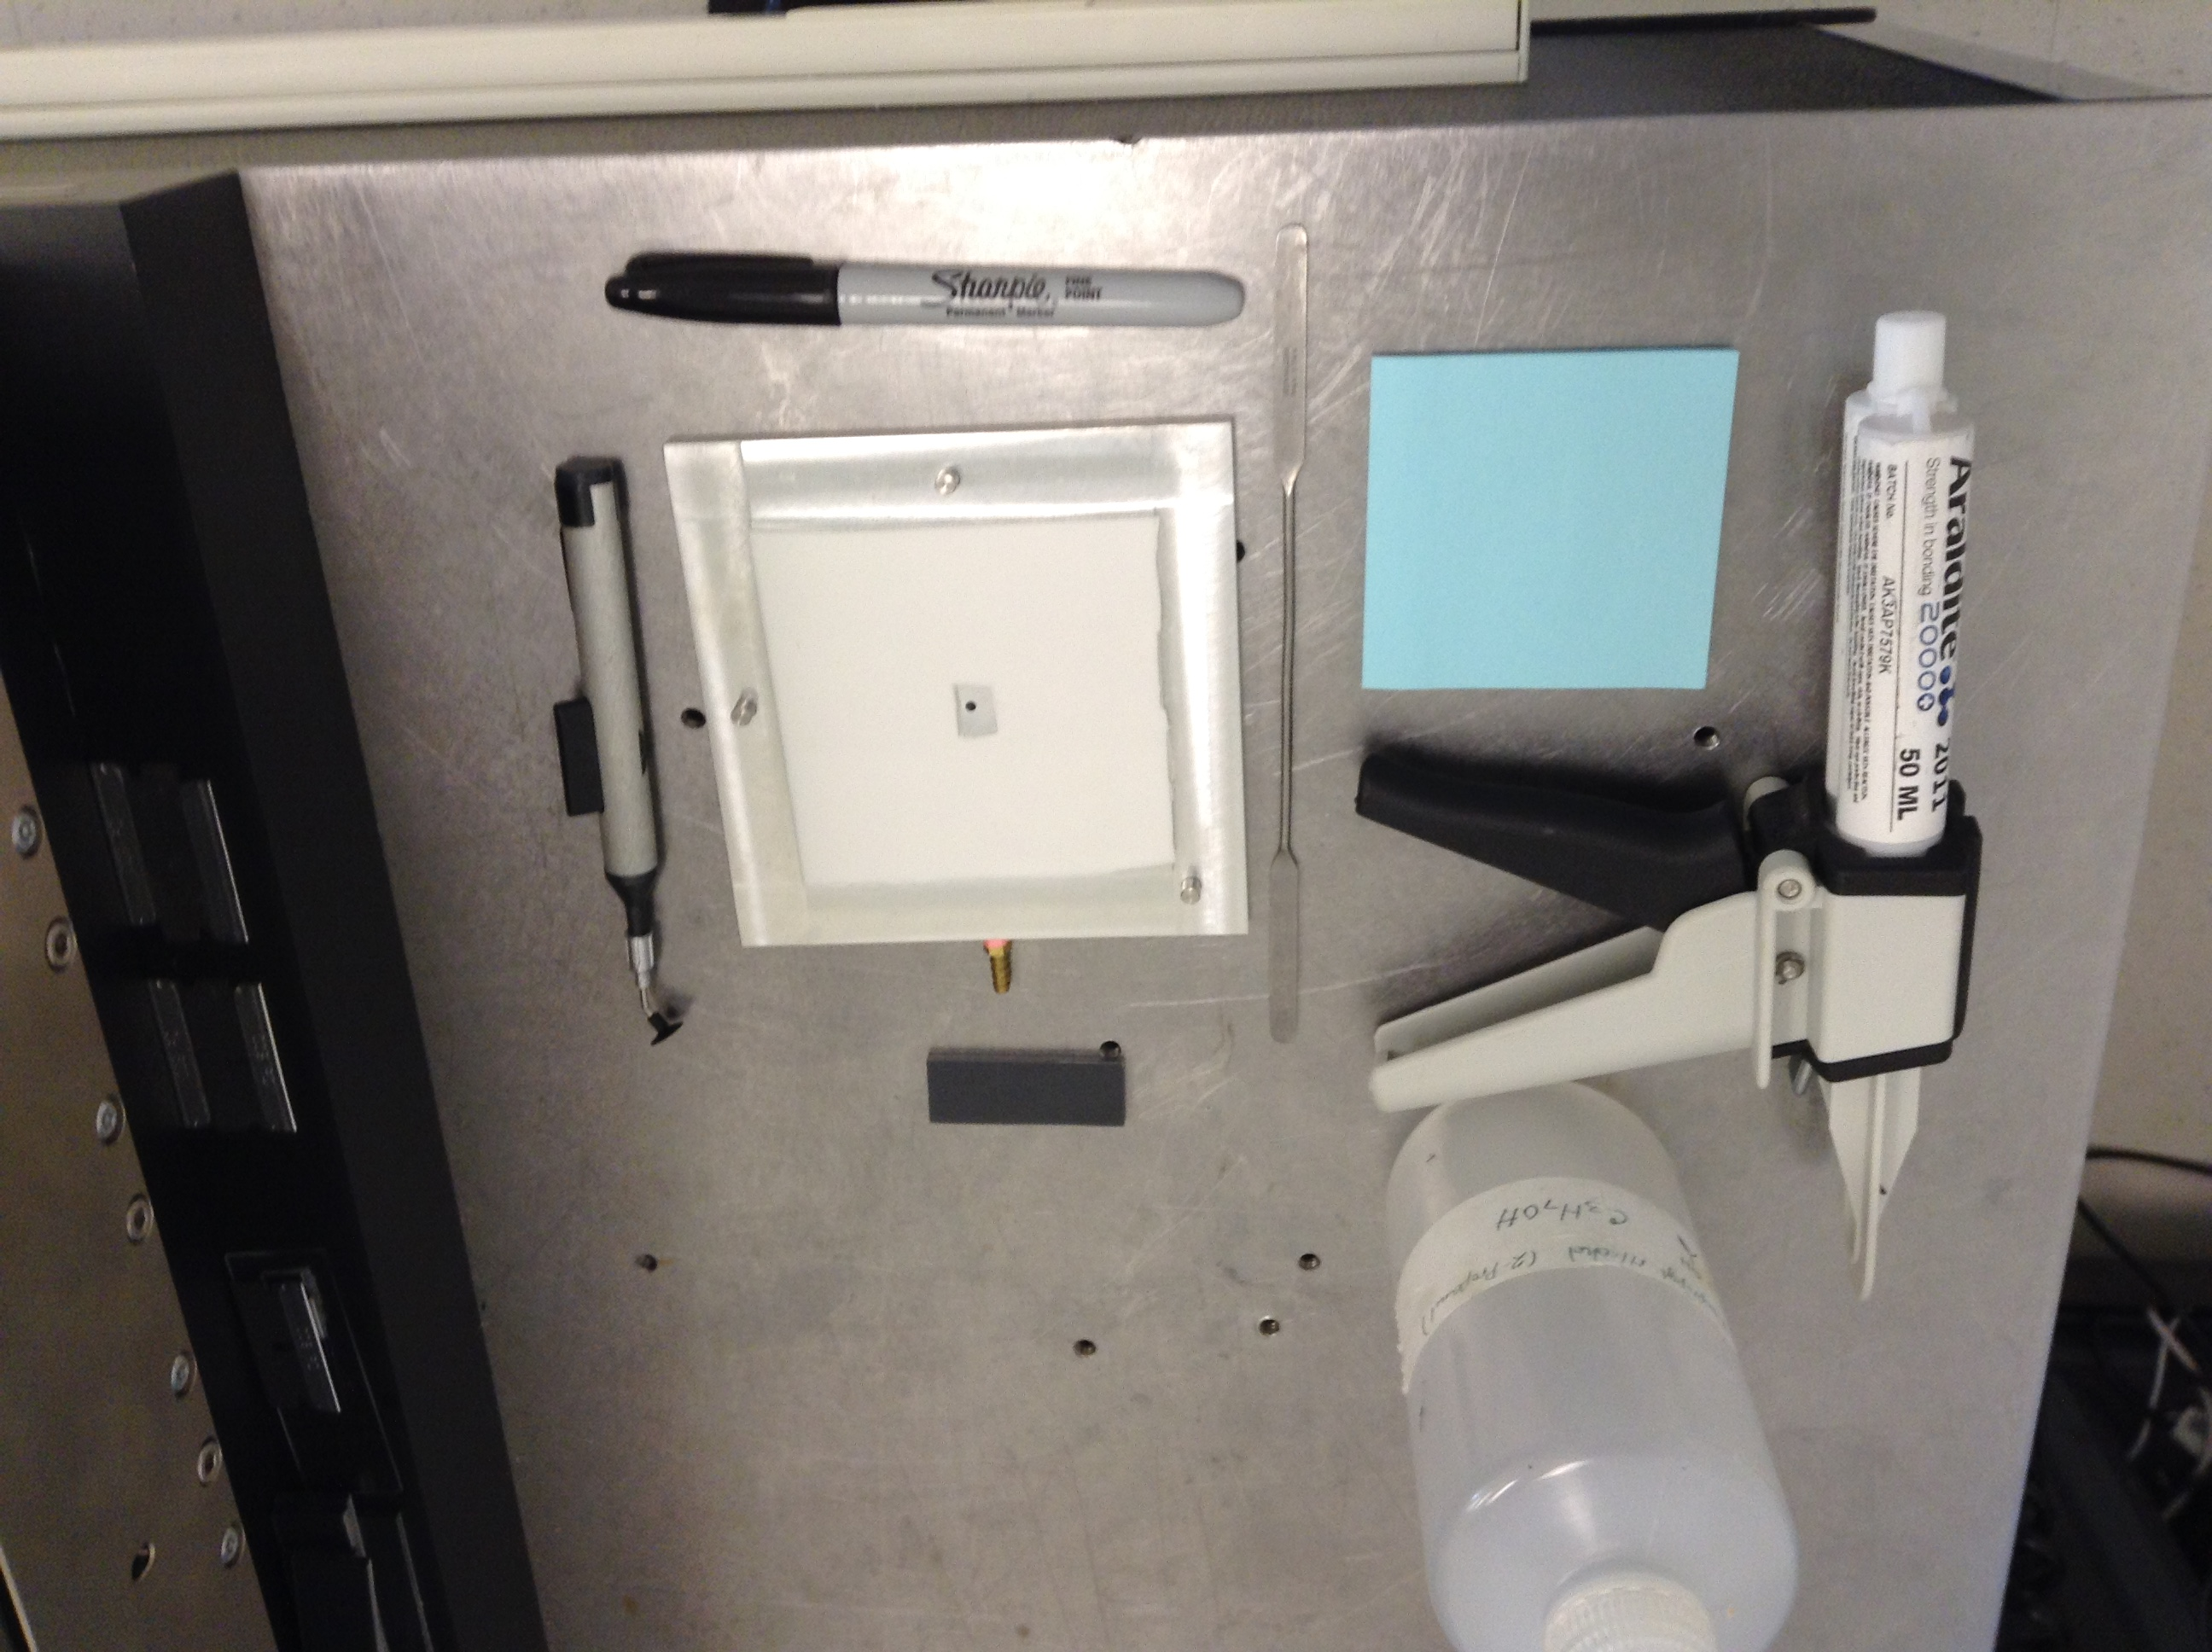
\includegraphics[width=0.9\textwidth,angle = -180]{img/gluingMaterials.jpg}
\caption{Materials used in the gluing process. These materials are located on the Gantry table, except for the cleaning materials which are located by the sink outside the clean room.}
\label{materials}
\end{figure}
\end{center}


Note: the arrangement may vary as long as it matches the setup in the software

%------------------------------------------------------------------
\section{Procedure}

\begin{enumerate}
    \item Perform a readiness check of the gantry:
    \begin{enumerate}
        \item Test presence of vaccum on the gauge, record the pressure.
        \item Open LabView control software ``Glueing\_V\#(main)''  where $\#$ is the software version. In the Desktop, there is a shortcut to the ``routine'' directory; in there find the directory ``Glueing V\#''. Use the latest version. Record version.$$ \sim\backslash MyDocuments\backslash andres\backslash routine\backslash glueing\_V\#\backslash Glueing\_V\#(main)$$
        \item Check the controller and power supply are turned on.
    \end{enumerate}
    \item Pick parts from storage (dry air cabinet) and identify them. Handle bare modules only with proper protection: ESD wristband, gloves, face mask. Check that the parts satisfy the quality criteria by retrieving their information in the database.
    \item Assign a new batch number (\texttt{Nxxx}) and assign a unique number (\texttt{Nxxxyy}) according to the rule described in \texttt{SOP~000}.
    \item Write the batch number to the BBM chuck on an edge for further identification.
    \item Open and run the LabView program `` vacuum manifold'' located at $$ \sim\backslash MyDocuments\backslash andres\backslash routine\backslash vacuum_manifold.vi$$
    \item Unplug the vacuum line connected to the glue reservoir chuck and plug it to the vacuum tool. 
    \item Repeat the following steps for the number of modules to be glued, as needed:
    \begin{enumerate}
        \item Remove clip from GelPak and place the GelPak onto the vacuum tool. Turn vacuum line \# 14 on. This allows the BBM to be removed with minimal force.
        \item Place the BBM on the chuck. Check if it is correctly aligned with the stencil.
        \item Place the HDI on the chuck. Check if it is correctly aligned with the stencil.
        \item Place at minimum the required number of stamp tools and weight tools on the respective chucks.
    \end{enumerate}
    \item If the GelPaks became empty, mark them as used and put them in the non-dry air cabinet. Otherwise return to the dry air cabinet.
    \item Plug back the vacuum line to the glue reservoir chuck.
    \item Run the control sotfware $(Glueing\_V\#(main))$ and provide the information required in the pop-up windows:
    \begin{enumerate}
        \item Adjust configuration in software to reflect positions in use.
        \item identification of the HDI's and modules.
    \end{enumerate}
    \item Run pattern recognition step (find fiducials button). Check if locations found are sound (statistical information in the front panel must be used for this purpose). The image showed as template gives an idea of what to look for. \\\\ 
      Supervise progress and stop if needed (using the RED stop button in the joystick), especially when modules are at risk.
    \item Prepare Araldite:
    \begin{enumerate}
        \item Record batch number of Araldite.
        \item Place a hazelnut-sized amount of Araldite (syringe provides both components at once) on Post-It note.
        \item Mix glue for one minute using the spatula.
        \item Place a portion of the glue on all the required positions of the glue reservoir. Evenly distribute and smoothen the surface using the disposable PVC squeegee.
        \item Coarsely clean spatula, dispose off Post-It note and squeegee.
    \end{enumerate}
    \item Run apply glue step (glue button). Some choices have to be done through pop-up windows. Comments and observations can be written anytime during the step execution.
    \item Run pick and place step (pick \& place button). Some choices have to be done through pop-up windows. Comments and observations can be written anytime during the step execution.
    \item Run pattern recognition after glue step (find fiducials after gluing button). Some choices have to be done through pop-up windows. Comments and observations can be written anytime during the step execution.
    \item Run put weight step (weight button). Some choices have to be done through pop-up windows. Comments and observations can be written anytime during the step execution.
    \item Run the finish step. (finish button). Final comments and observations can be written in a pop-up window.
    \item Press the ``create report and finish'' button to generate the final report; some information have to be provided in a pop-up window.
    \item At the end of the full cycle, remove chuck with stamp tools and clean them thorougly using water and 2-propanole at sink outside the cleanroom. Let them dry and bring back to gantry.
    \item Document all actions even if the curing time may not be over. For this, do the following steps for each module glued:
    \begin{enumerate}
        \item Select the BBM from the parts list: ``MAIN MENU''$\rightarrow$``Part List'' and click on the corresponding BBM in the ``Bare Module'' table.
        \item Click on the link ``Update Status''.
        \item Select the checkbox ``HDI attached'', select the HDI that has been glued onto that module.
        \item Enter your name in the ``User'' field
        \item Enter the UNL batch number for this module in the ``Comments'' field. Add any other observations.
    \end{enumerate}
    \item Finished modules shall not be handled for at least 2~hours.
    \item Weight tools may be removed using the gantry after 2~hours of curing time but modules need to remain protected from any mechanical stress for a total curing time of 10~hours.
    \item At the discretion of the operator, the remaining curing time can take place off the gantry provided the modules are still placed on the original chuck, on a level surface inside the cleanroom. The storage cabinets are not suitable for this (outgasing of glue). Such removal from the gantry needs to be documented.
    \item If the wirebonding doesn't happen within a few hours after the curing time is over, transfer the chuck into the dry air cabinet.
    \item Inform the wirebond technicians about the fact that new modules are available for wirebonding.
\end{enumerate}

%------------------------------------------------------------------
\section{Documentation}
The following information is recorded in the report generated by the glueing software:
\begin{itemize}
    \item Date, time (start--end) and operator name
    \item LabView software: version
    \item Id of parts used:
	\begin{itemize}
	    \item HDI: S/N
	    \item BBM: identification on box plus identification according to naming convention
	    \item UNL batch number
	\end{itemize}
\end{itemize}

Find the report at $\sim\backslash MyDocuments\backslash andres\backslash routine\backslash reports$. Any special observations, e.g. damage to parts not already recorded during visual inspection, deviations from normal procedures, can be added to the report, just open it  and add the info. Publish it in the UNL elog. 

\end{document}

